\chapter{PCA Filters in Layer 1}
\begin{figure}[h] 
  \begin{center}
   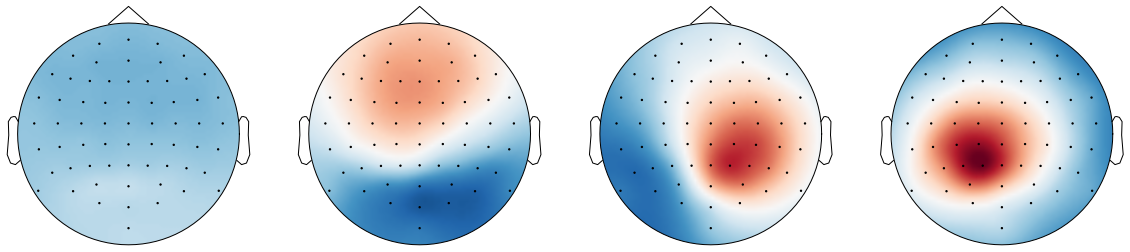
\includegraphics[width=.5\textwidth,keepaspectratio=true]{Figures/PCA_SVM}
   \\\vspace{-0.8em}
    \caption{PCA done on training trials}
    \label{fig:PCA_SVM}
  \end{center}
  \vspace{-1em}
\end{figure}

\begin{figure}[h] 
  \begin{center}
%  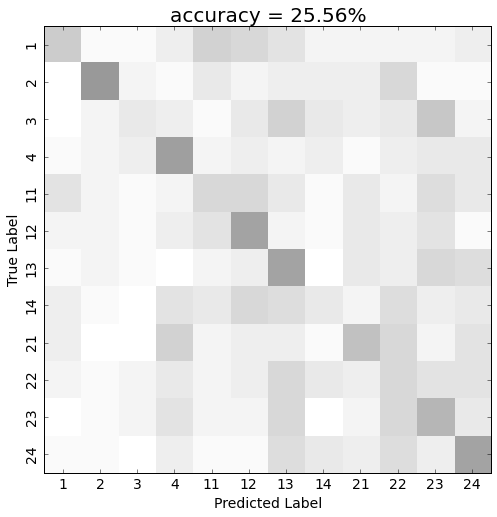
\includegraphics[width=.5\textwidth,keepaspectratio=true]{Figures/PC0_confusion}
    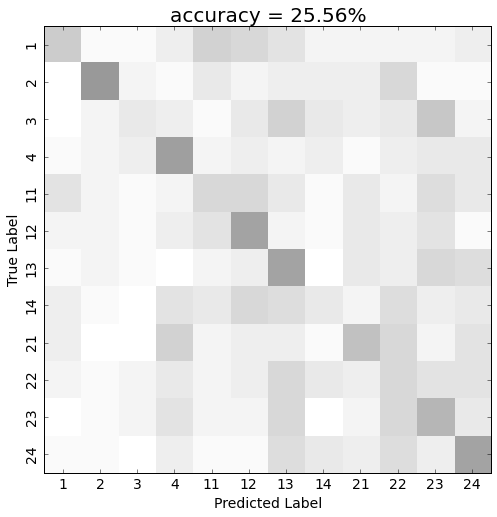
\includegraphics[scale=0.5]{Figures/PC0_confusion}
   \\\vspace{-0.8em}
    \caption{Replacing layer 1 with PC 0}
    \label{fig:PC0_confusion}
  \end{center}
  \vspace{-1em}
\end{figure}

\begin{figure}[h] 
  \begin{center}
%    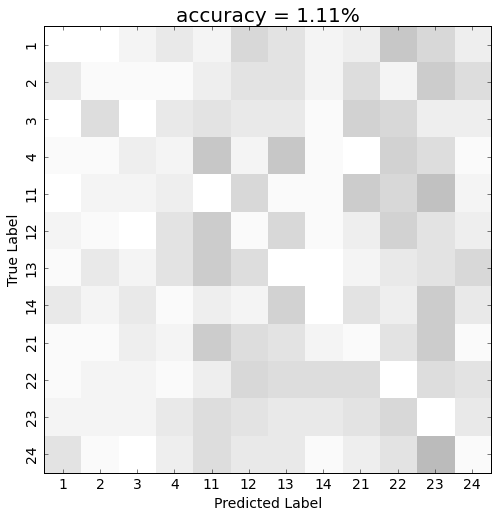
\includegraphics[width=.5\textwidth,keepaspectratio=true]{Figures/PC1_confusion}
    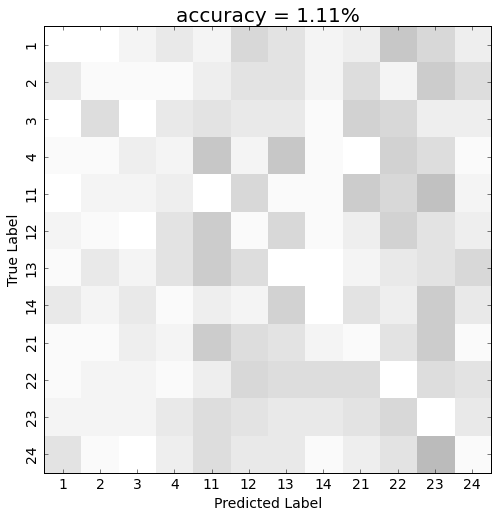
\includegraphics[scale=0.5]{Figures/PC1_confusion}
   \\\vspace{-0.8em}
    \caption{Replacing layer 1 with PC 1}
    \label{fig:PC1_confusion}
  \end{center}
  \vspace{-1em}
\end{figure}

\begin{figure}[h] 
  \begin{center}
%    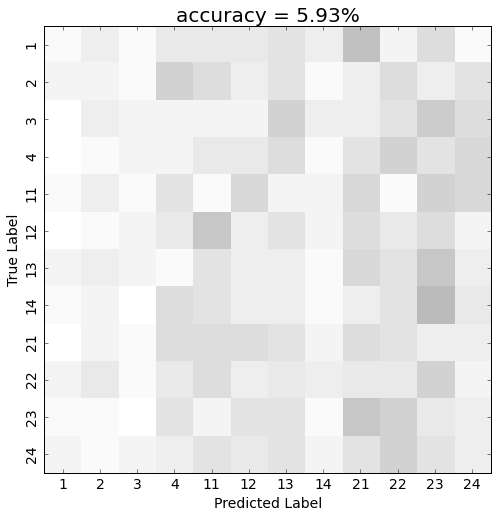
\includegraphics[width=.5\textwidth,keepaspectratio=true]{Figures/PC2_confusion}
    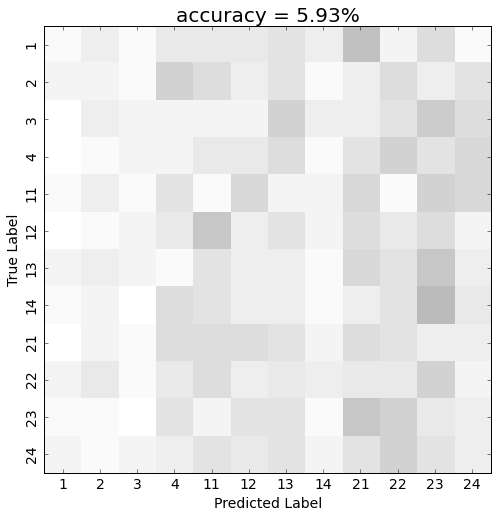
\includegraphics[scale=0.5]{Figures/PC2_confusion}
   \\\vspace{-0.8em}
    \caption{Replacing layer 1 with PC 2}
    \label{fig:PC2_confusion}
  \end{center}
  \vspace{-1em}
\end{figure}

\begin{figure}[h] 
  \begin{center}
%    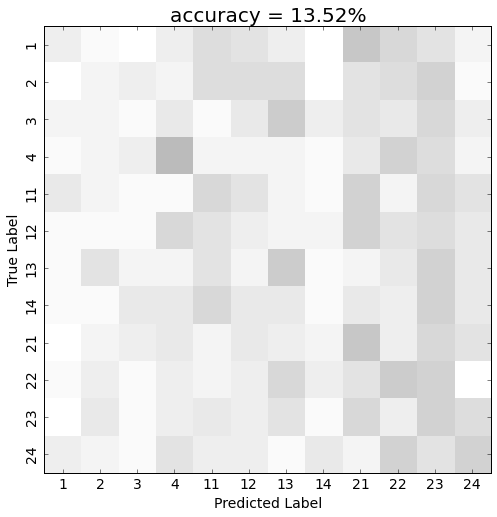
\includegraphics[width=.5\textwidth,keepaspectratio=true]{Figures/PC3_confusion}
    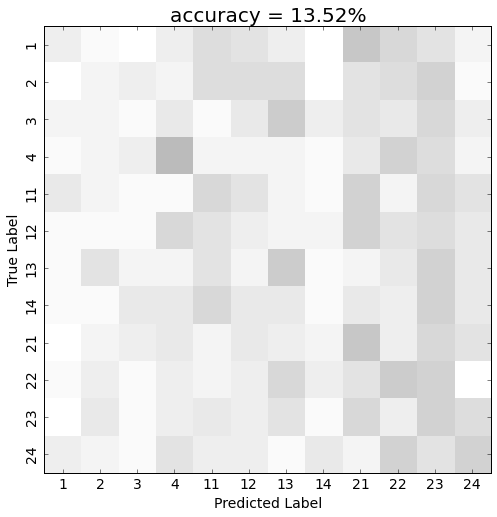
\includegraphics[scale=0.5]{Figures/PC3_confusion}
   \\\vspace{-0.8em}
    \caption{Replacing layer 1 with PC 3}
    \label{fig:PC3_confusion}
  \end{center}
  \vspace{-1em}
\end{figure}